\chapter{Ispitivanje}
Ispitani su sustavi za napajanje, komunikacije između dijelova sustava, bežična komunikacija, upisivanje korisničkog programa u Flash memoriju mikrokontrolera, snimanje zvuka, pohrana podataka na SD karticu, RTC, komunikacija s PPG senzorom i mjerenje impedancije kože.

U svim testovima korišten je multimetar za mjerenje napona i osciloskop za promatranje signala u komunikacijama između sustava. Za ispitivanje napajanja korišteni su USB strujni adapter koji podržava mogućnost brzog punjenja, razne litij-ionske baterije u 18650 kućištu i USB ispitivač UT658DUAL tvrtke Changan UNI-T prikazan na slici \ref{slk:UT658DUAL}. Ovaj uređaj se može spojiti između USB izvora i uređaja te pokazuje razinu napona, jakost struje koju izvor daje, količinu potrošenog naboja u mAH i vrijeme trajanja mjerenja.
\begin{figure}[htb]
    \centering
    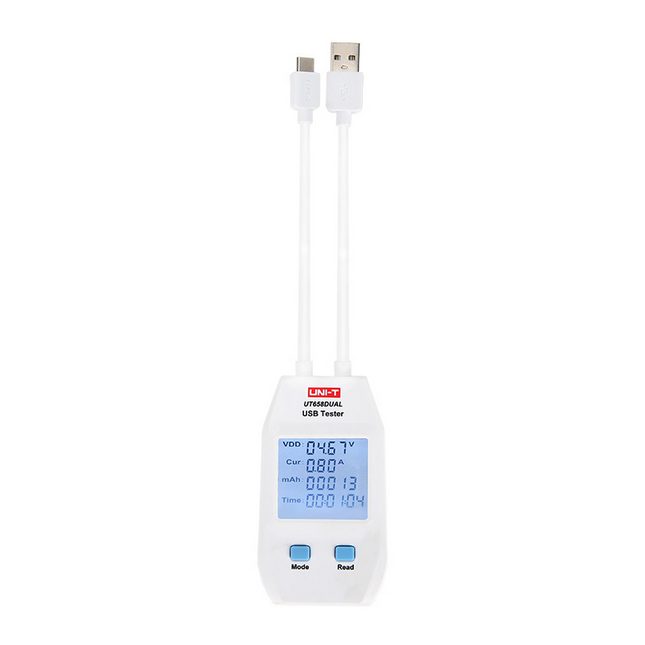
\includegraphics[width=6 cm]{Figures/UT658DUAL.png}
    \caption{USB ispitivač UT658DUAL}
    \label{slk:UT658DUAL}
\end{figure}
\section{Središnji uređaj}
Na slikama \ref{slk:MB_TEST_01} i \ref{slk:MB_TEST_02} prikazano je ispitivanje središnjeg uređaja. Umjesto priključka za bateriju namontiran je držač za standardnu 18650 bateriju radi lakšeg testiranja. Naime, baterija se često vadi i stavlja tijekom testiranja, a odabran priključak je predviđen da se rijetko otkapča, pa ga je radi toga i teško otkopčati.
\begin{figure}[htb]
    \centering
    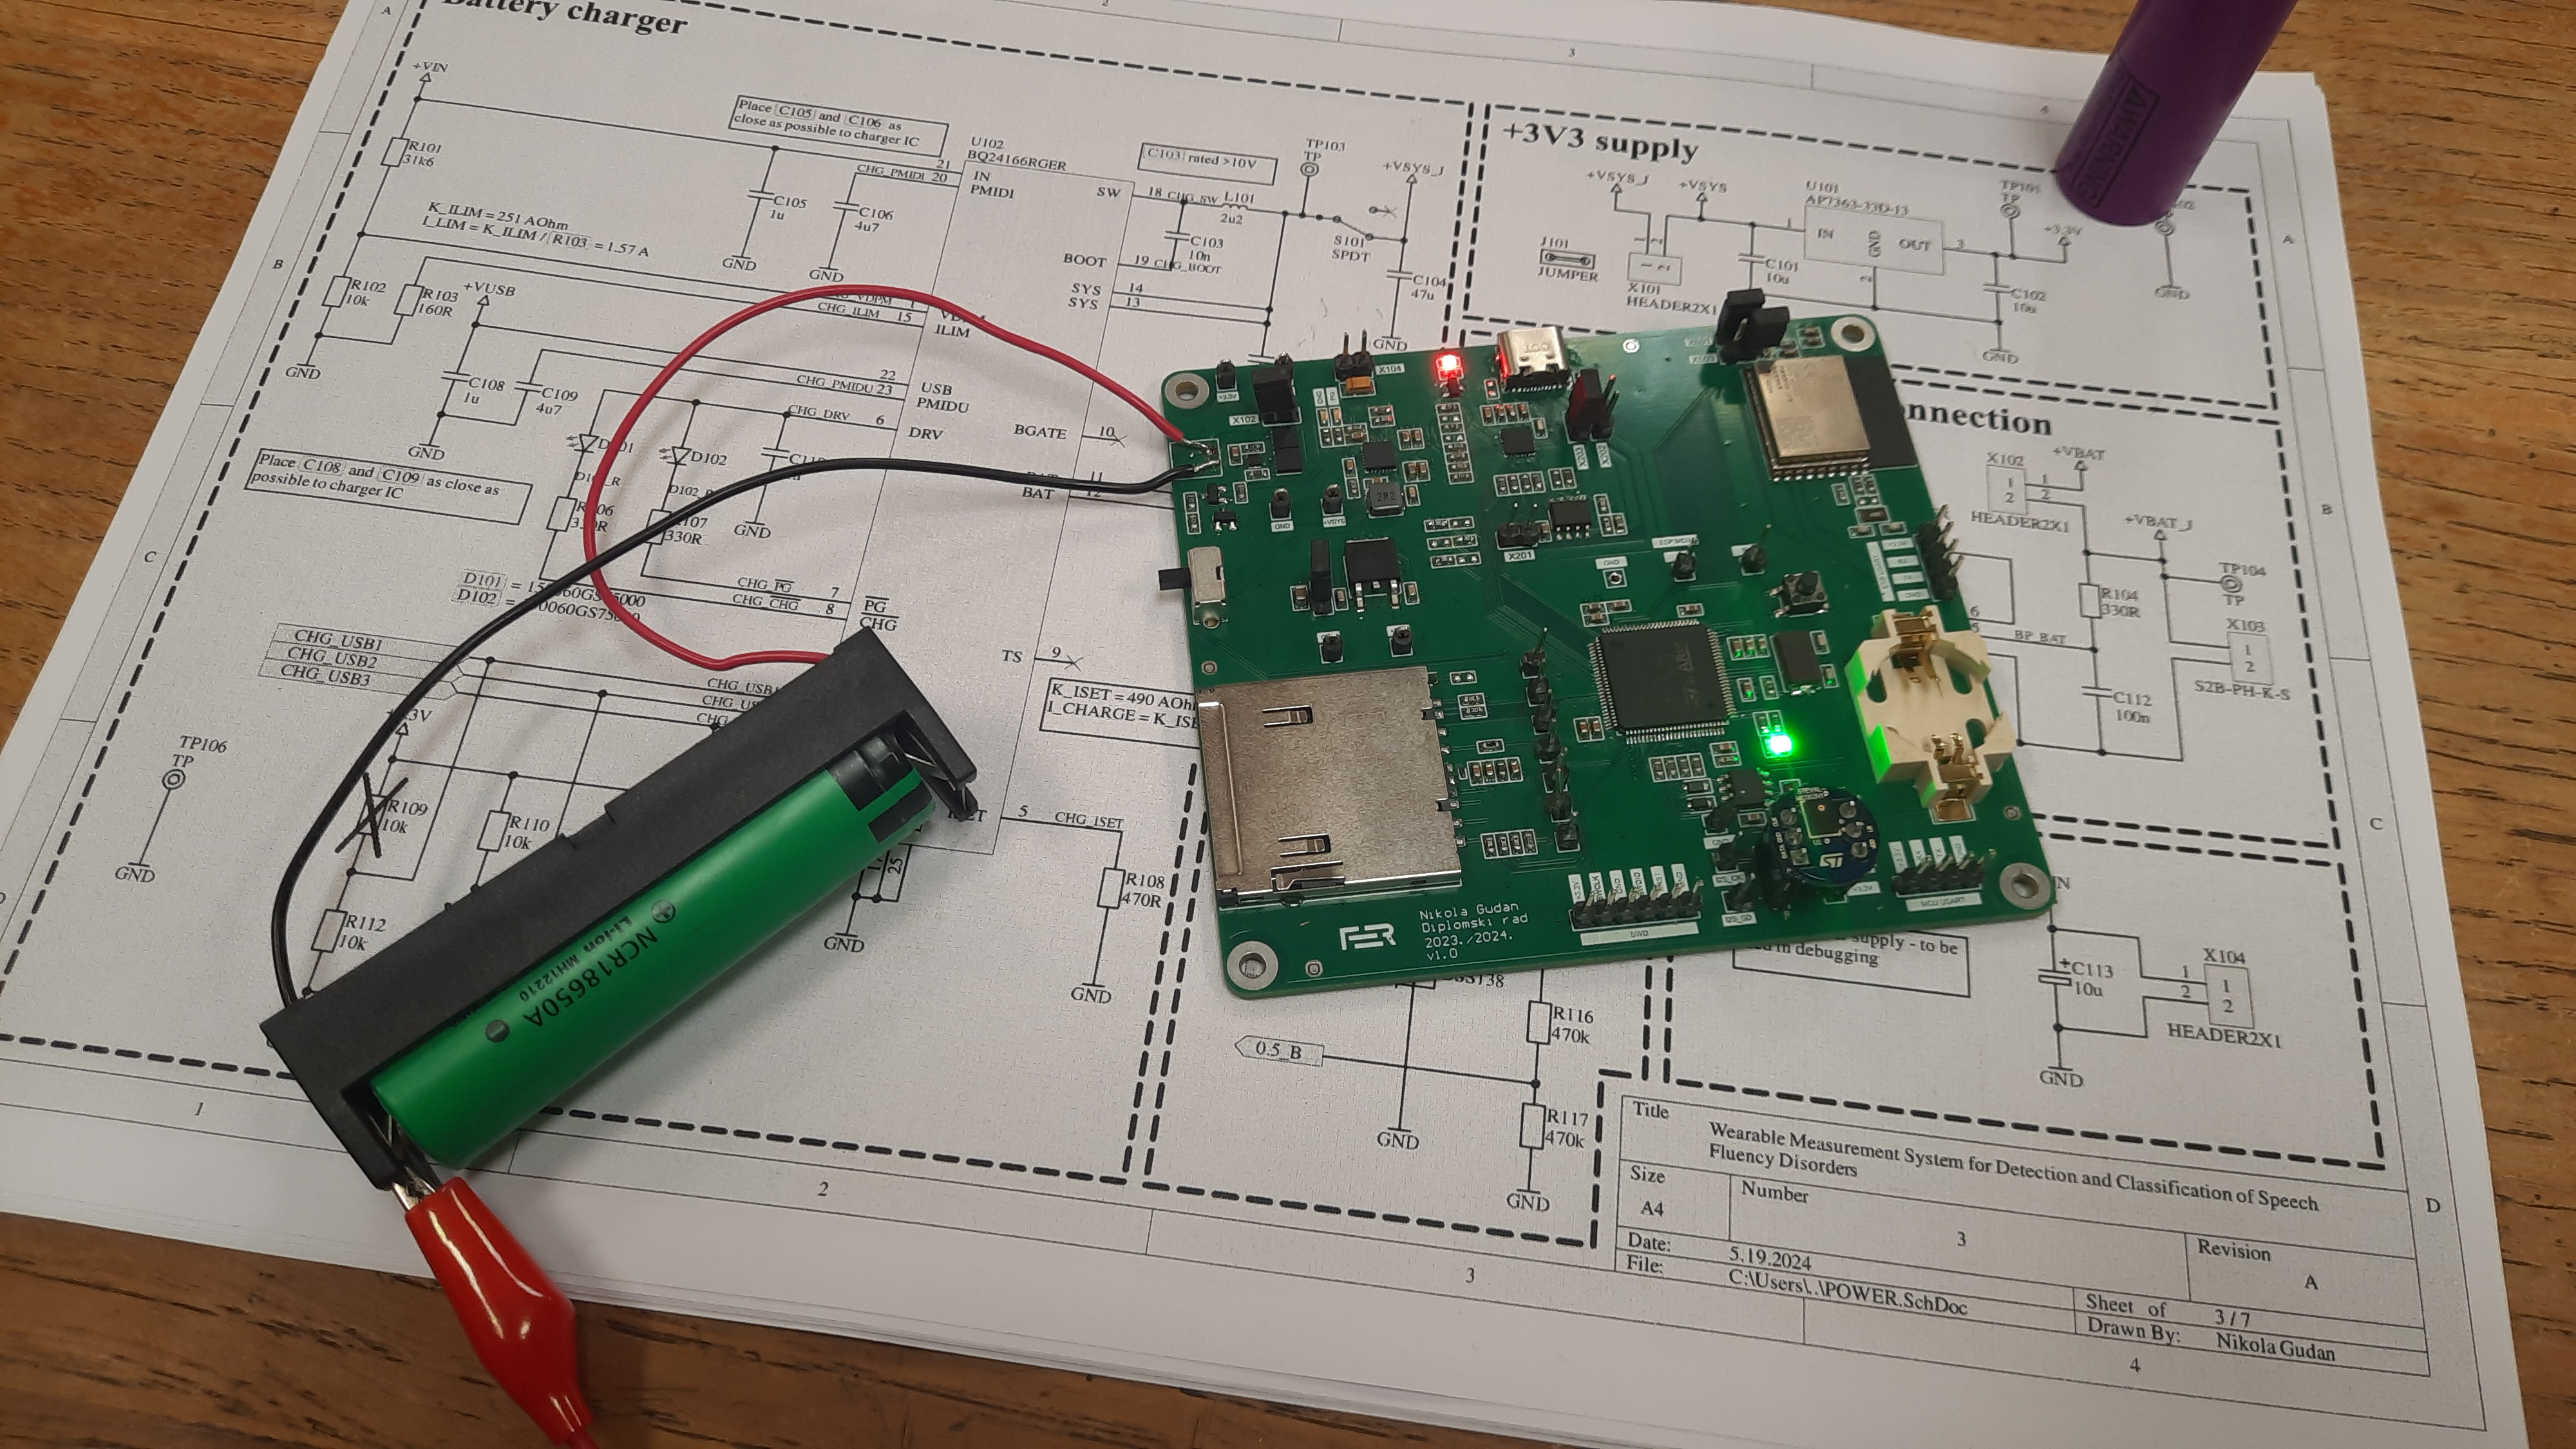
\includegraphics[width=10 cm]{Figures/MB_TEST_01.jpg}
    \caption{Ispitivanje pločice središnjeg uređaja}
    \label{slk:MB_TEST_01}
\end{figure}
\begin{figure}[htb]
    \centering
    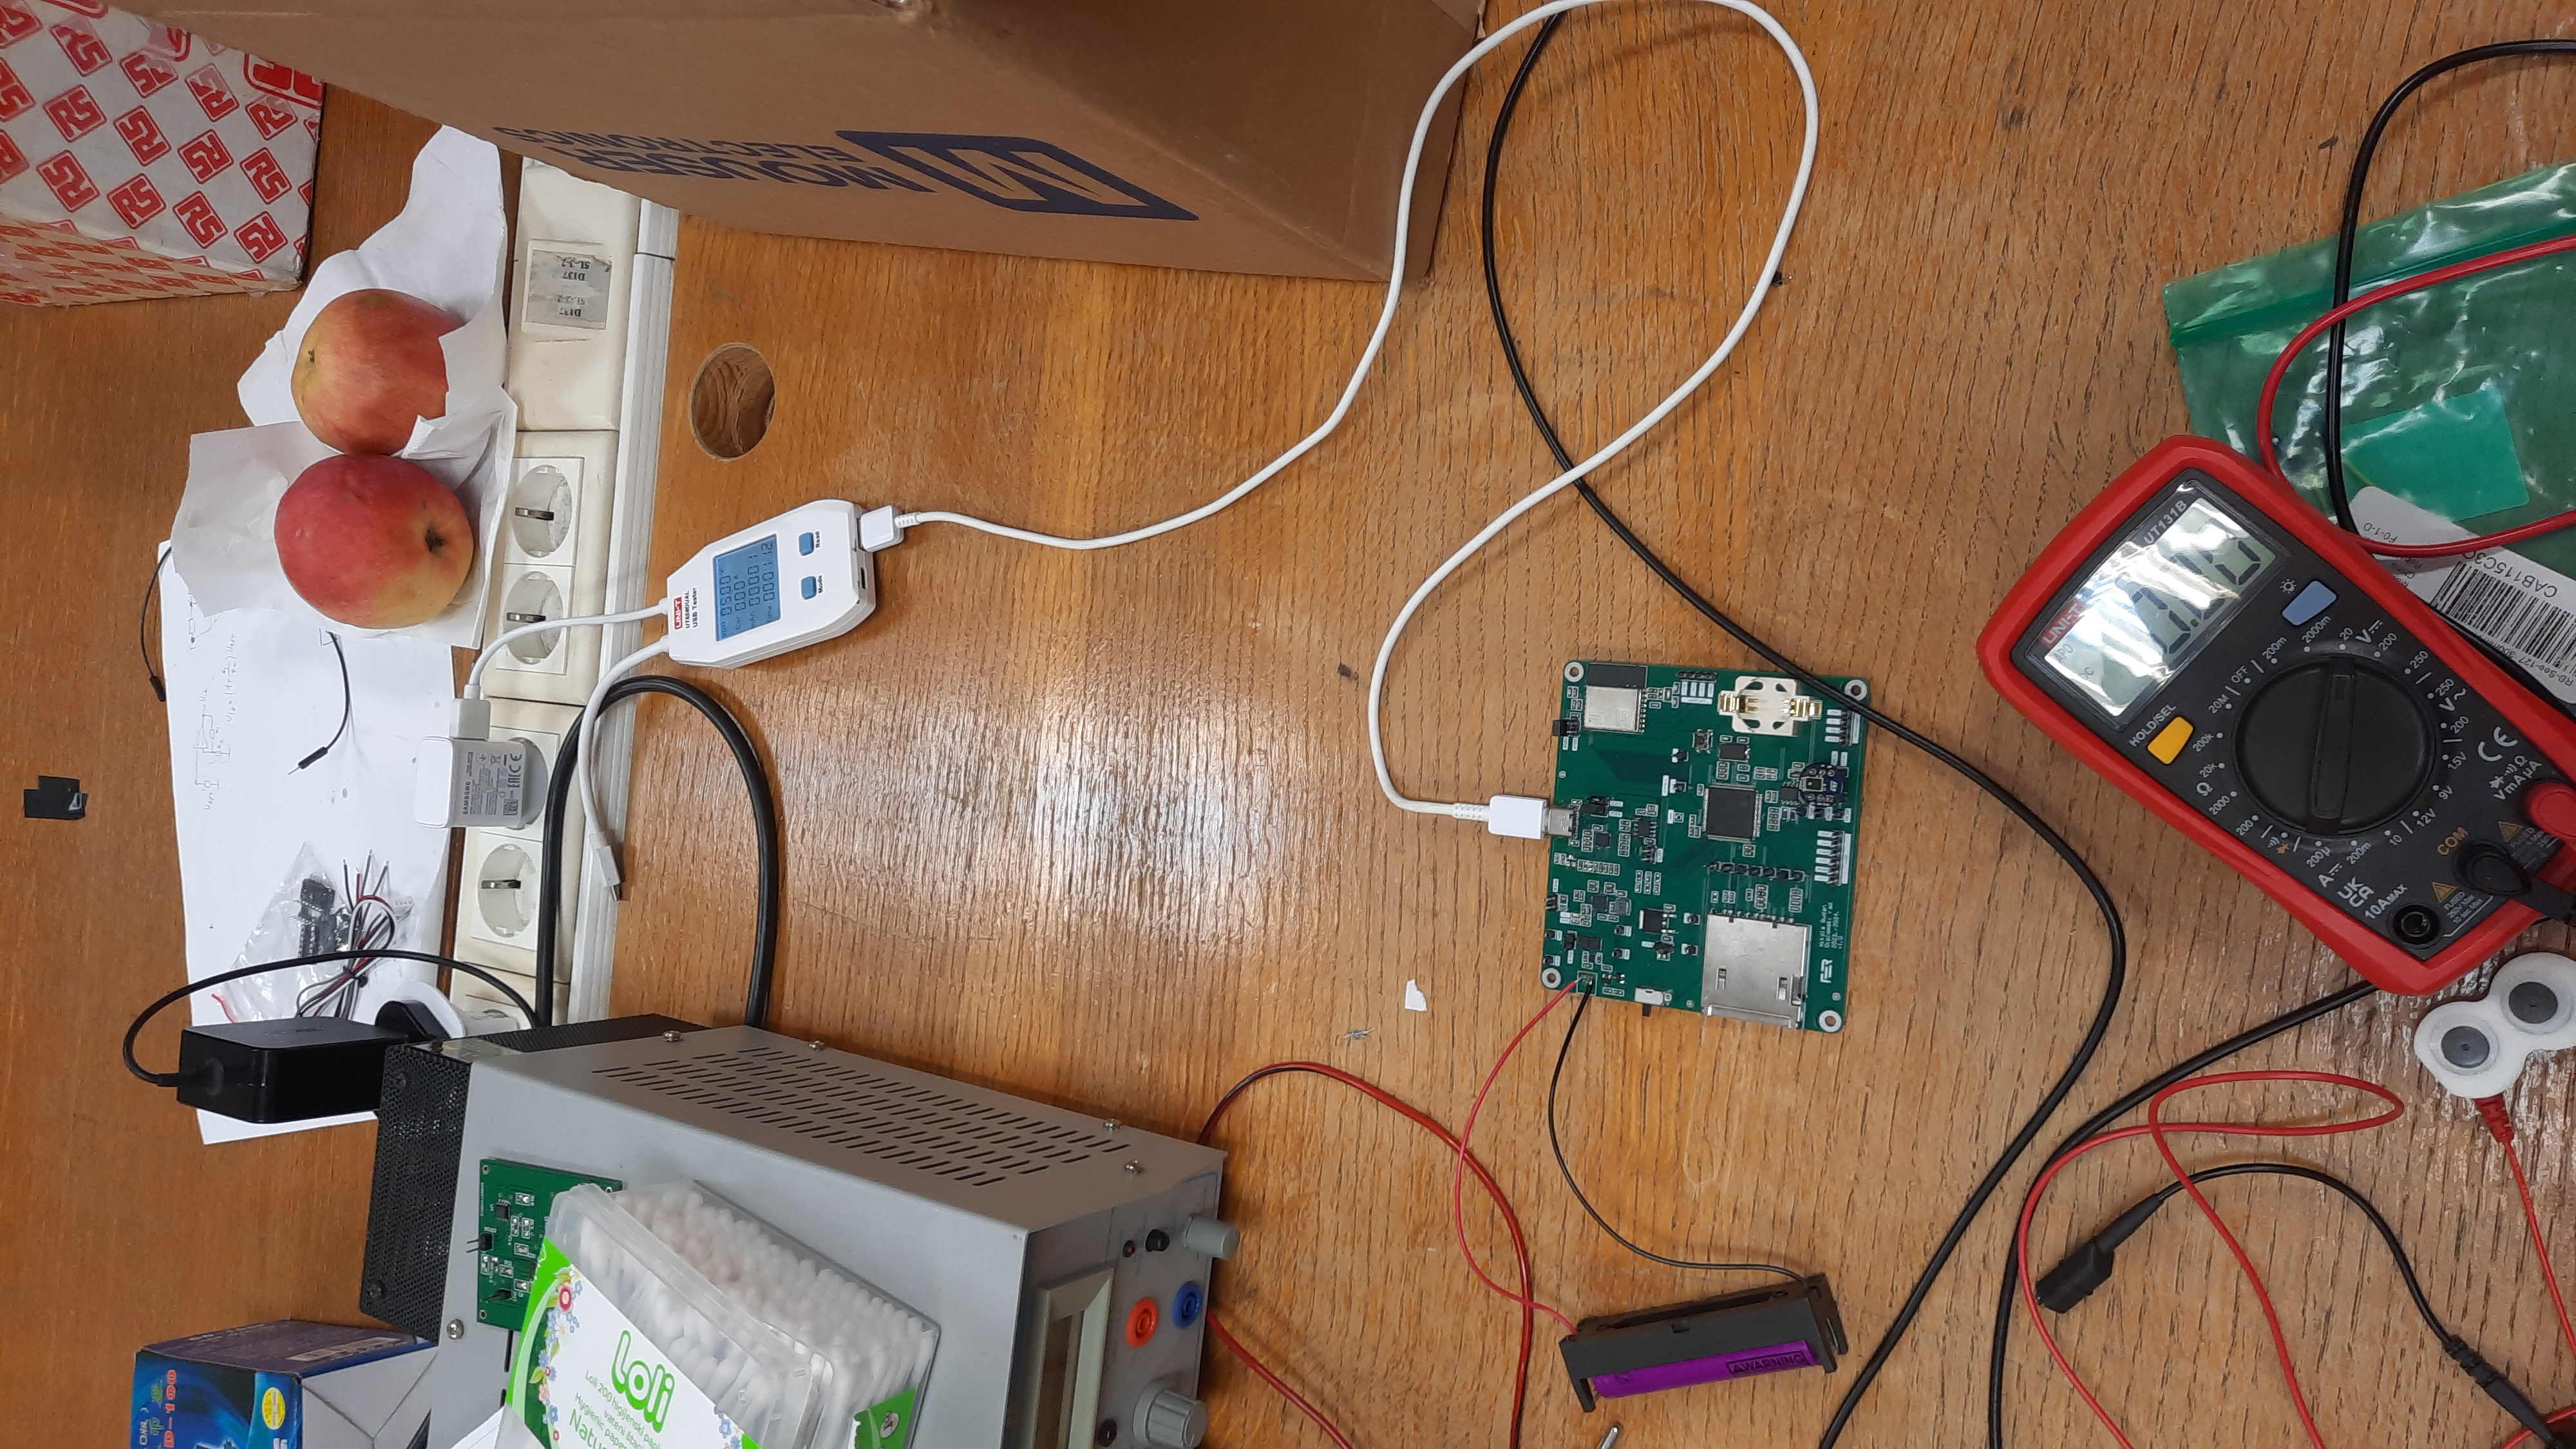
\includegraphics[width=10 cm]{Figures/MB_TEST_02.jpg}
    \caption{Postav ispitivanja pločice središnjeg uređaja}
    \label{slk:MB_TEST_02}
\end{figure}

Oktrivena je greška u dizajnu USB napajanja. Kada se spoji USB, bez obzira na to da li izvor podržava zatraženu snagu ili ne, napajanje sa USB-a se ne prosljeđuje dalje na ostatak sustava. Problem se nalazi u tranzistorskoj sklopci (slika \ref{slk:MB_USB}). Naime, kada čip pokuša uključiti tranzistore, na prvom tranzistoru dolazi do pada napona na porednoj diodi koja se nalazi unutar tranzistora, pa se na uvodu drugog tranzistora nalazi napon napajanja umanjen za napon provoda diode (između 0.5 V i 1.2 V \cite{di:dmp3098}). Čip je preko VDC\_OUT stezaljke onda detektirao prevelik pad napona i onemogućio napajanje sa USB-a. Radi toga su napravljene izmjene u USB napajanju kod narukvice vidljive na slici \ref{slk:BR_USB}.

Kada baterija nije bila spojena, nije bilo moguće uključiti USB napajanje iz razloga objašnjenog u potpoglavlju \ref{sec:BR_USB}. Ukratko, čip nije mogao postaviti odgovarajuće otpornike na CC linije pa se nije mogla zatražiti nikakva snaga od USB izvora.

Tijekom testiranja punjača utvrđeno je da punjač može bez problema proslijediti napon baterije na izlaz. Međutim, kada se je priključio vanjski napon, bilo na USB ili preko priključka za laboratorijski izvor napona u svrhu punjenja baterije, punjač više nije radio. Bilo je vidljivo trepteranje svjetlećih dioda za indikaciju ispravnog napajanja i punjenja u frekvenciji 1 treptaj po sekundi. Naime, dolazi do aktiviranja temperaturne zaštite na način opisan u potpoglavlju \ref{sec:BR_BATCHG}.

Tijekom čekanja izrade tiskane pločice, razvijena je cjelokupna programska podrška za središnji uređaj. S obzirom na to da većina napajanja, izuzev baterije, nije radila, tijekom testiranja programske podrške, a samim time i digitalnog dijel sustava, uređaj se je napajao preko programatora, koji je bio priključen na pločicu cijelo vrijeme tijekom testiranja programske podrške. Utvrđeno je da mikrofon normalno snima govor, mikrokontroler komunicira sa svim podsustavima te također bez poteškoća obrađuje i sprema podatke na SD karticu, bežični podsustav se uspješno može programirati i RTC mjeri vrijeme napajavši se sa litijske baterije. Dakle, digitalni dio sustava u potpunosti radi.

\section{Narukvica}

\begin{figure}[htb]
    \centering
    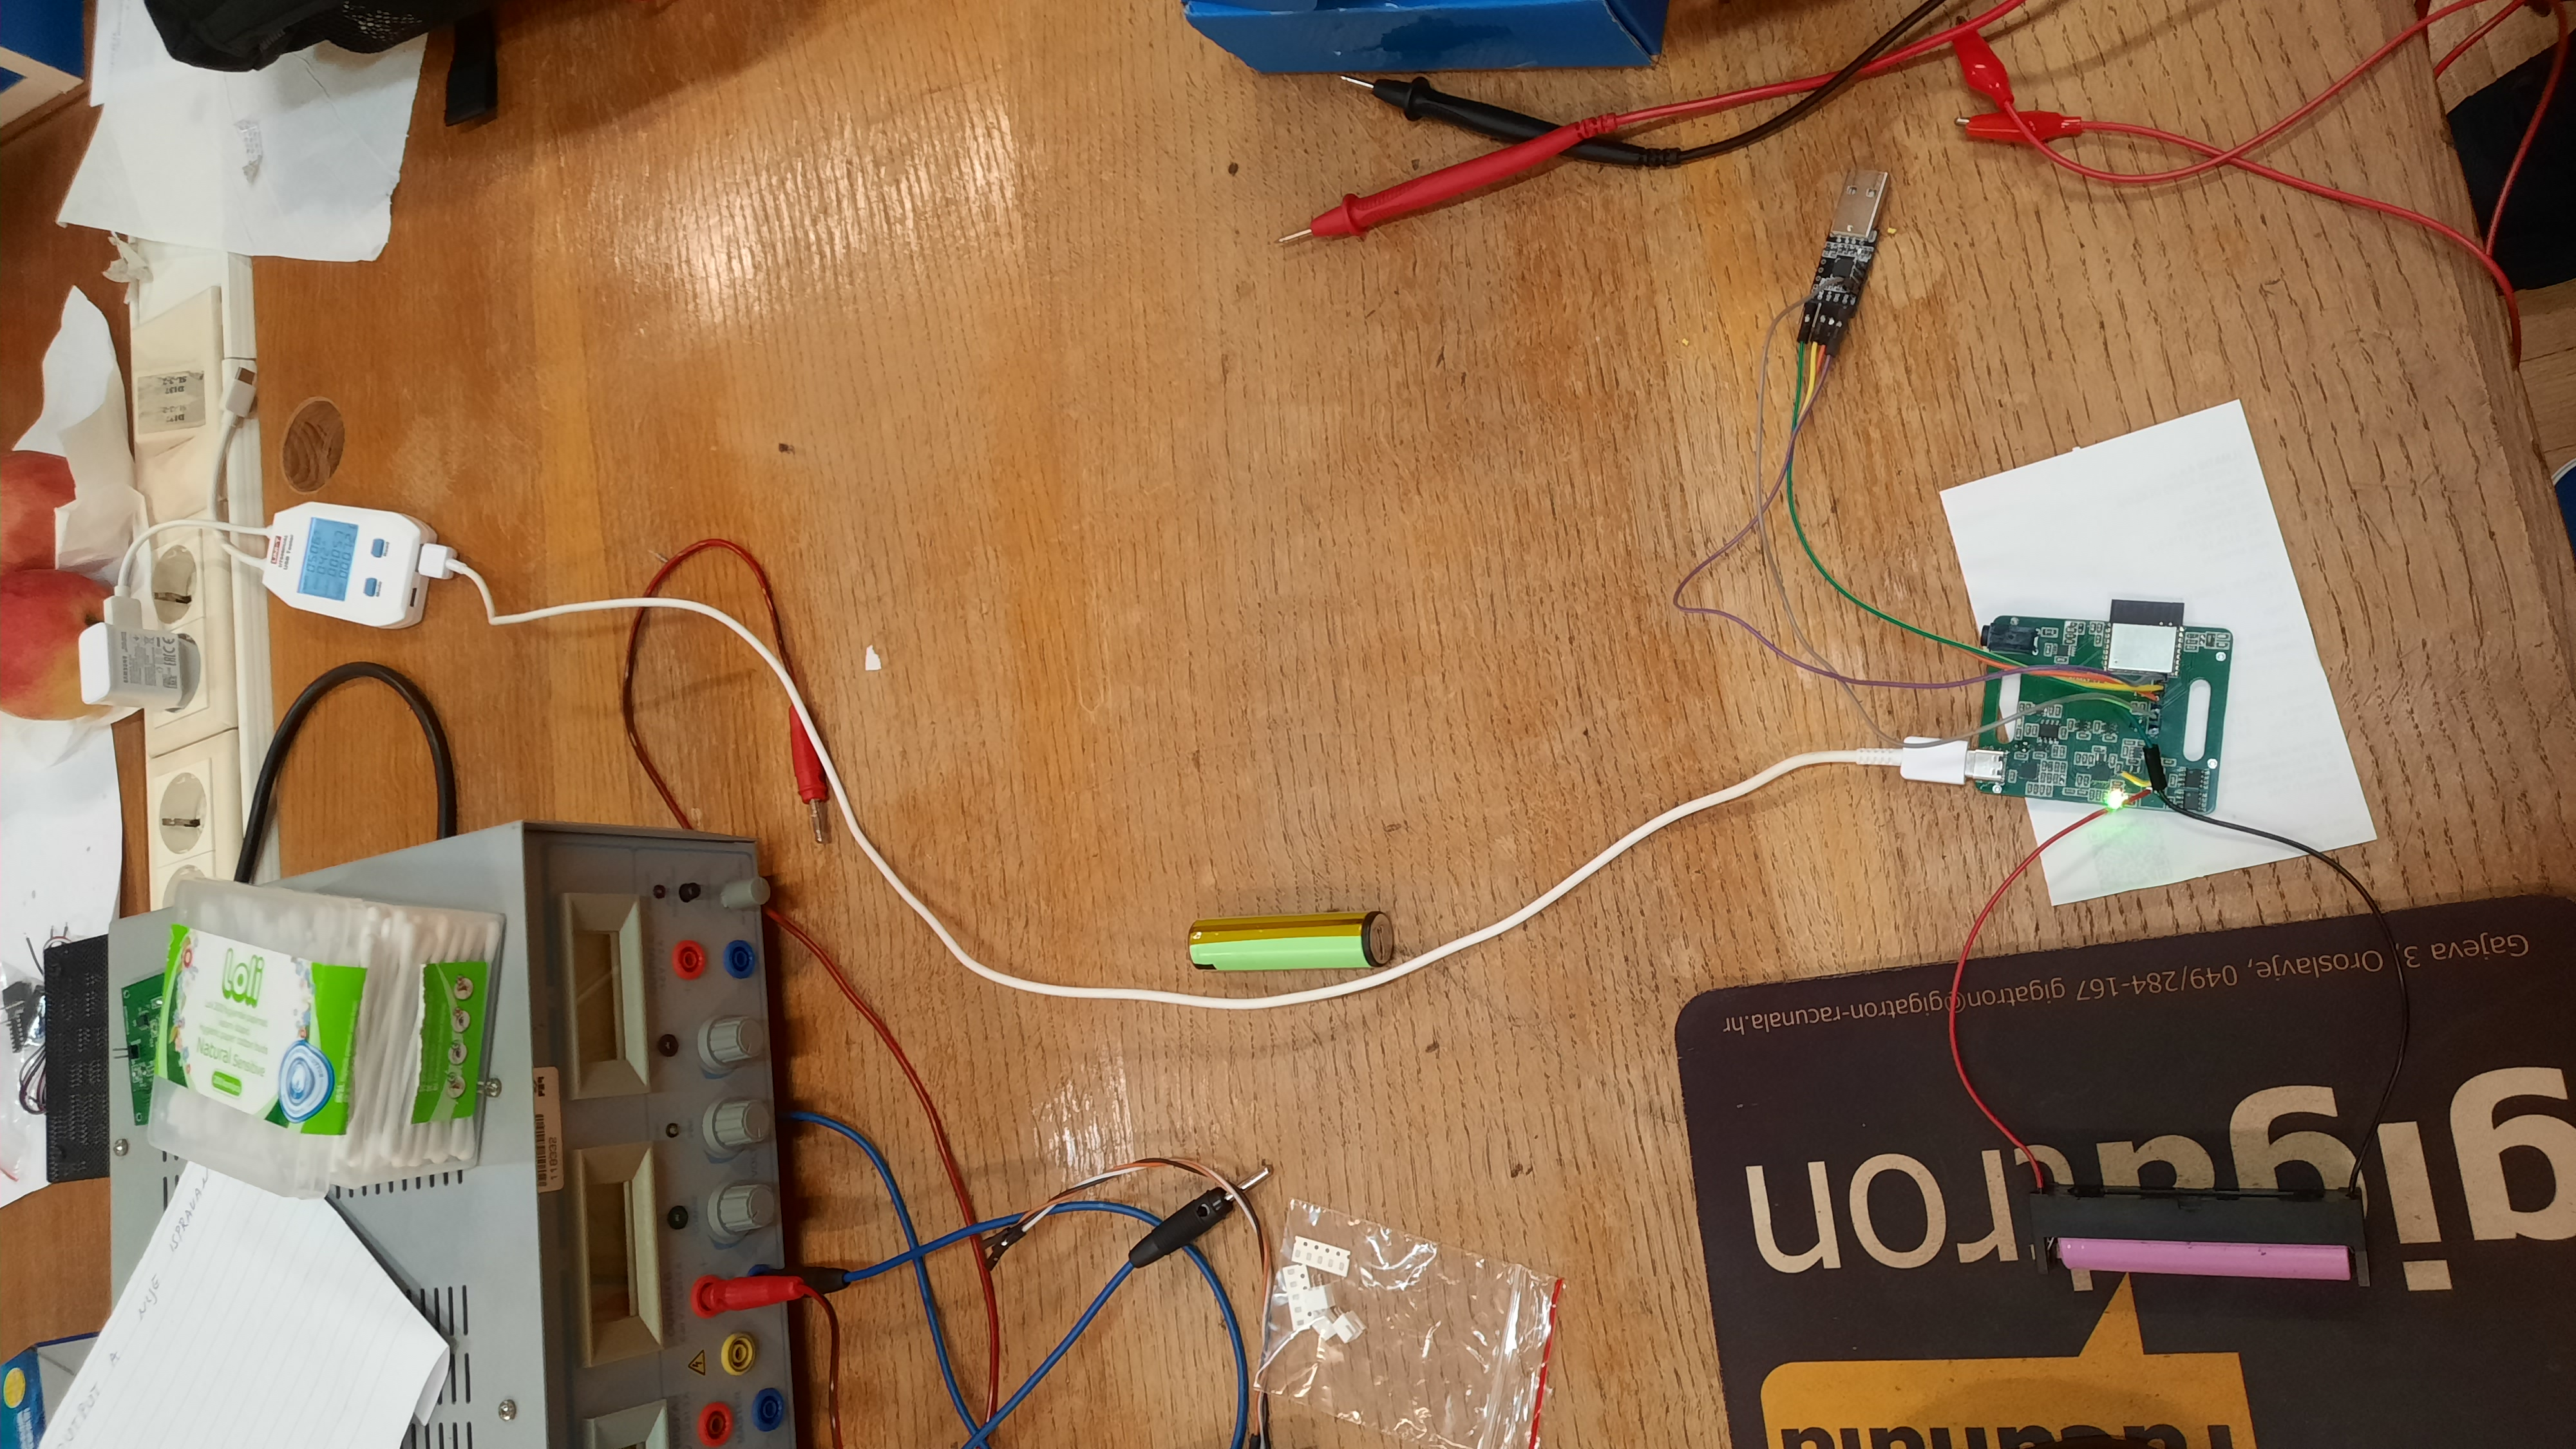
\includegraphics[width=10 cm]{Figures/BR_TEST_02.jpg}
    \caption{Postava ispitivanja pločice narukvice}
    \label{slk:BR_TEST_01}
\end{figure}
\begin{figure}[htb]
    \centering
    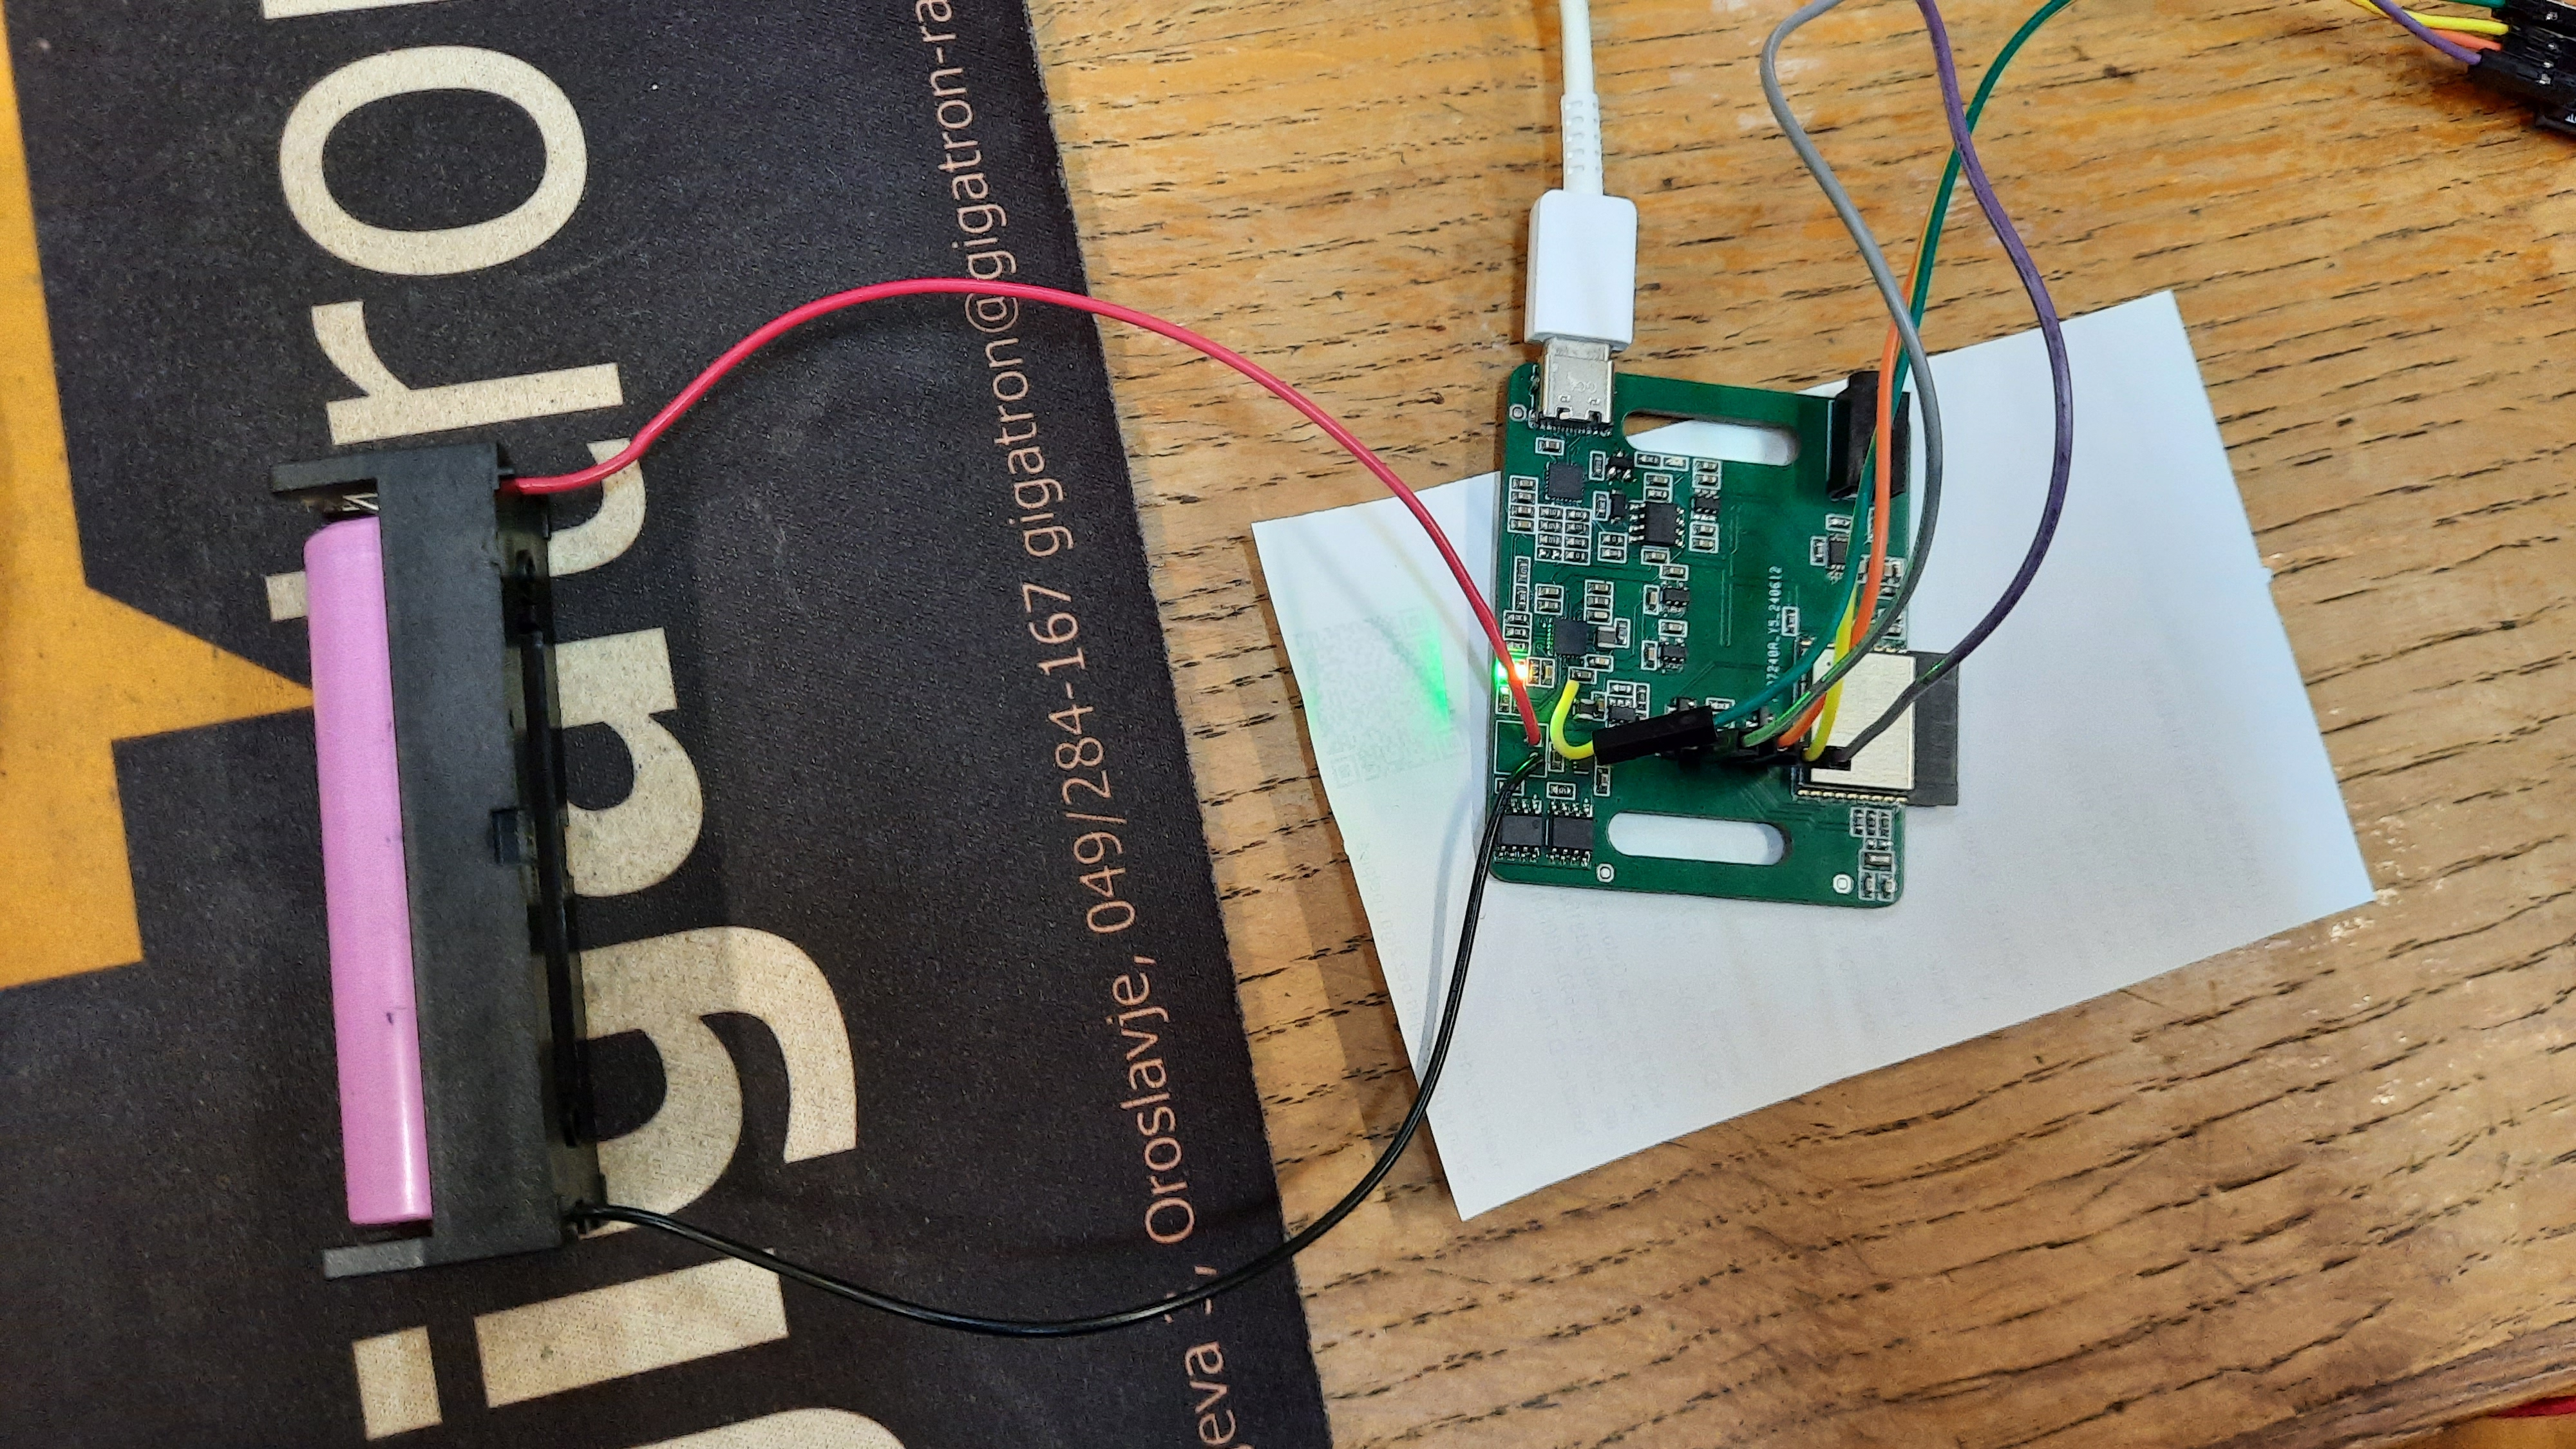
\includegraphics[width=10 cm]{Figures/BR_TEST_01.jpg}
    \caption{Ispitivanje pločice narukvice}
    \label{slk:BR_TEST_02}
\end{figure}

Na temelju ispitivanja središnjeg uređaja, napravljene su izmjene i popravci napajanja opisani u poglavlju \ref{pog:bracelet}. Prikaz ispitivanja se nalazi na slikama \ref{slk:BR_TEST_01} i \ref{slk:BR_TEST_02}.

Tijekom ispitivanja primjećena je greška u dizajnu baterijskog napajanja. Ime mreže koja je spojena na pozitivan terminal baterije (slika \ref{slk:BR_BATPROT}) i ime mreže koja je spojena na ulaz za bateriju na punjaču (slika \ref{slk:BR_BATCHG}) su različiti. Radi toga baterija, nakon zaštite, efektivno nije bila nigdje spojena, pa je bilo potrebno te dvije mreže kratko spojiti žicom.

Napajanje sada radi. Podsustav za USB napajanje sada može upravljati napajanjem i kada je na uređaj spojeno samo USB napajanje, a i cjelokupna narukvica se sada može napajati sa USB-a i kada baterija nije spojena. Baterijski punjač može proslijediti napajanje baterije ili može regulirati napajanje USB-a.
\begin{figure}[htb]
    \centering
    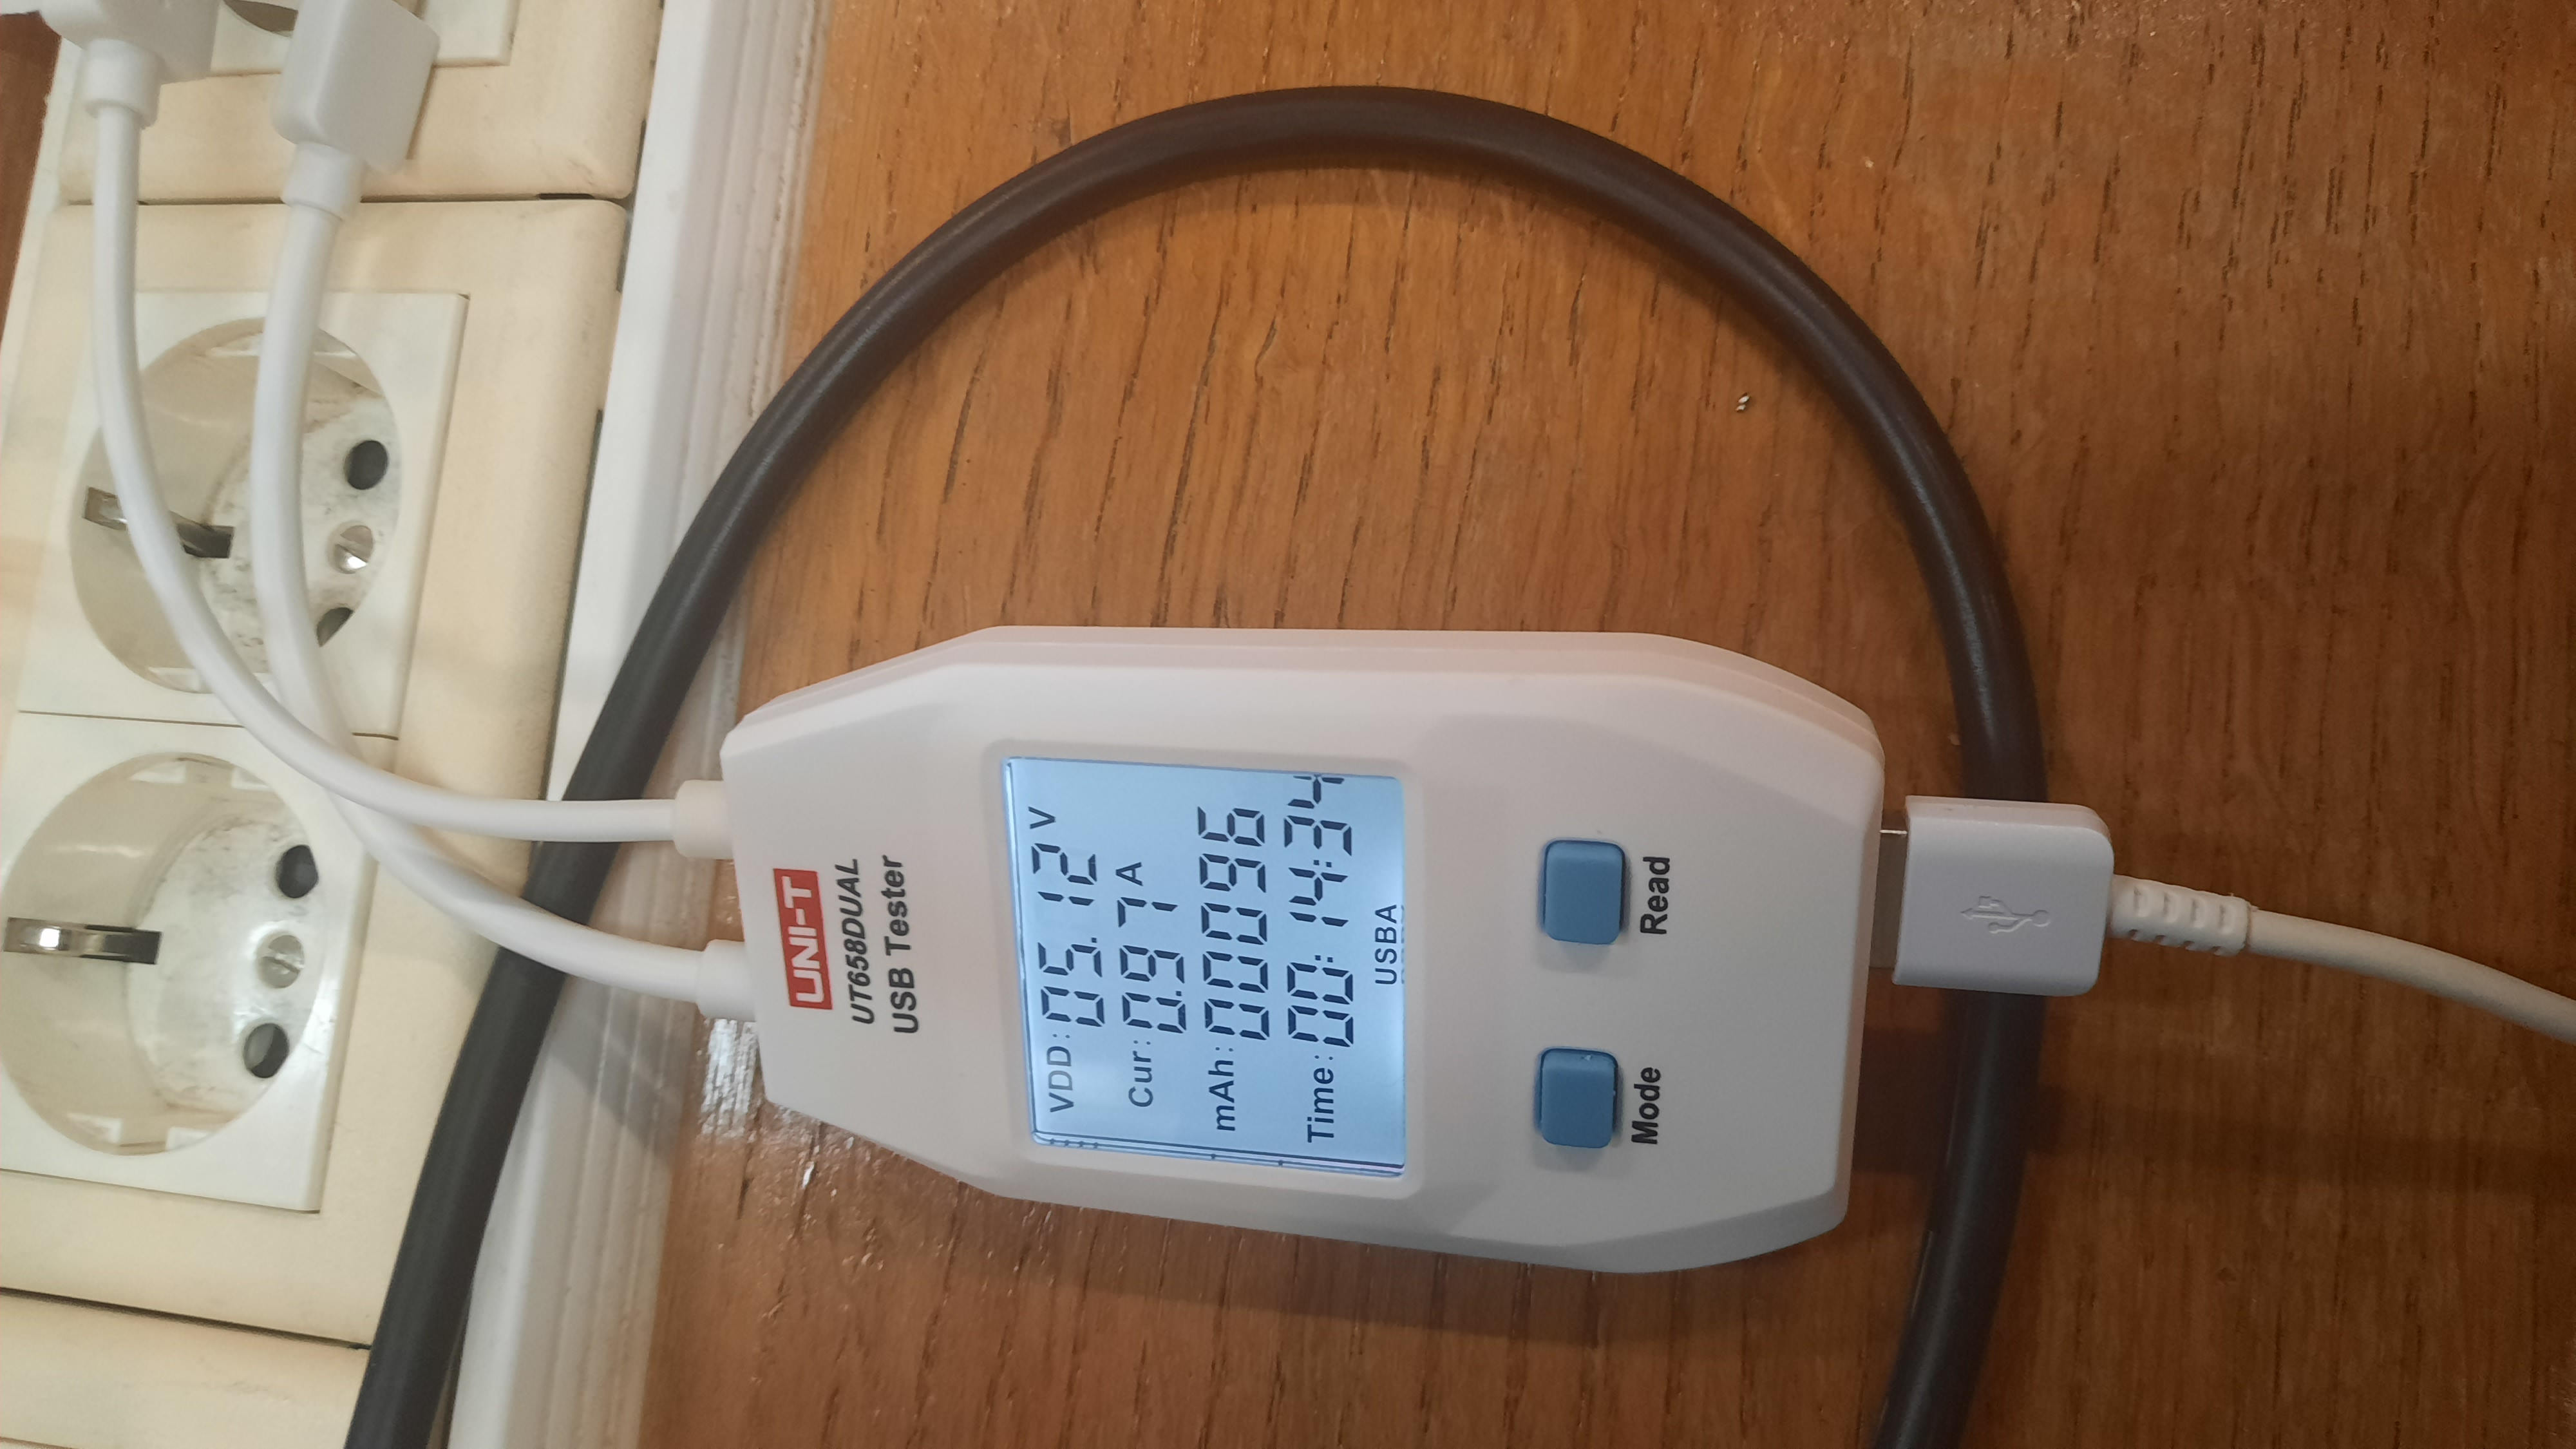
\includegraphics[width=10 cm]{Figures/BR_TEST_04.jpg}
    \caption{Brzo punjenje, punjenje konstantnom strujom}
    \label{slk:BR_TEST_04}
\end{figure}
\begin{figure}[htb]
    \centering
    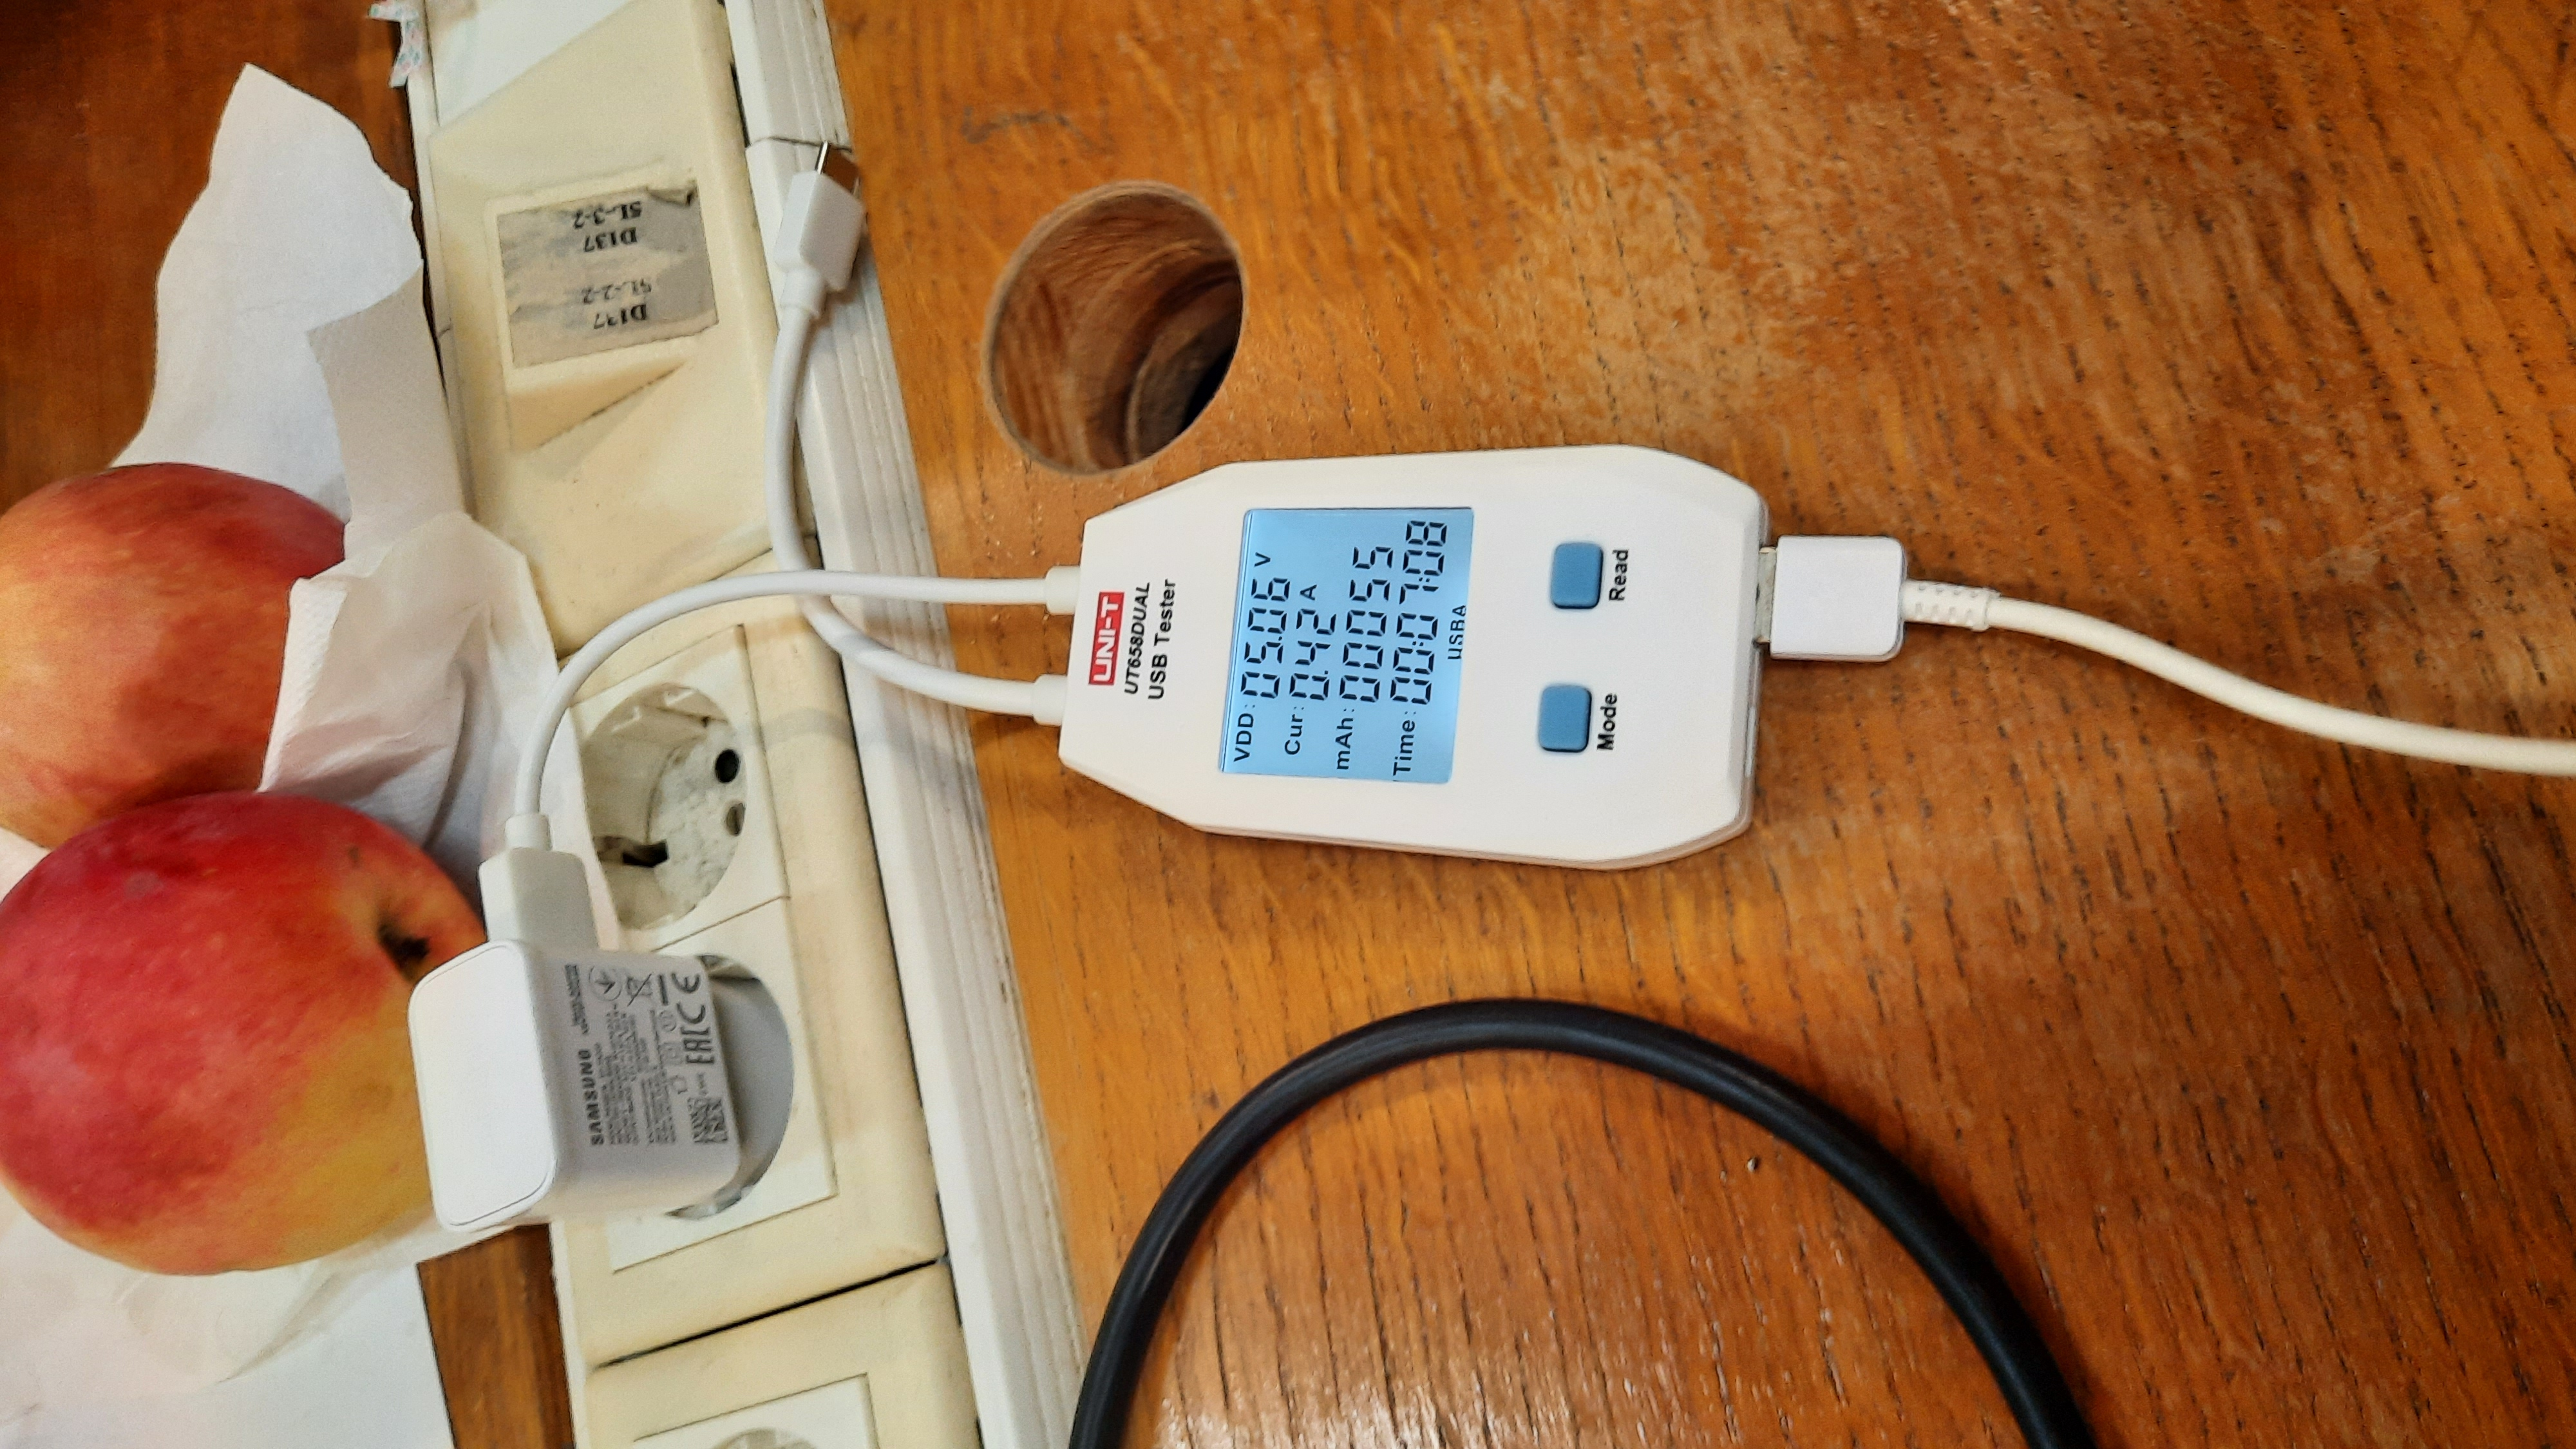
\includegraphics[width=10 cm]{Figures/BR_TEST_03.jpg}
    \caption{Brzo punjenje, punjenje konstantnim naponom}
    \label{slk:BR_TEST_03}
\end{figure}
Punjenje baterije konstantnom strujom i konstantnim naponom prikazano je na slikama \ref{slk:BR_TEST_04} i \ref{slk:BR_TEST_03}. Sustav ima napajanje i tijekom punjenja, dakle punjač sada isto radi. Prekidački i linearni regulatori provjereni su multimetrom i na svom izlazu pokazuju napon za koji su projektirani.

Tijekom ispitivanja mjernog lanca za EDR primjećeno je da je priključak za elektrode veoma loše kvalitete jer se je stalno gubio kontakt. Radi toga je taj priključak odlemljen, a žice za EDR su onda direktno zalemljene na pločicu. Još jedan problem je osciliranje pojačala, a to je rješeno preuzorkovanjem i usrednjavanjem više mjerenja sa ADC-a. Nakon toga su se dobivala stabilna mjerenja koja su odgovarala očekivanim rezultatima.

PPG senzor se nažalost nije mogao ispitati. Naime, tijekom montaže, gornji sloj pločice se je lemio pomoću infracrvene peći radi velike količine komponenata, dok je donji sloj lemljen pomoću vrućeg zraka. Senzor nije predviđen za montažu vrućim zrakom, pa se je tijekom lemljenja oštetio i otpalo je stakalce koje štiti diode i fotodetektor. Također nije bilo moguće provijeriti kvalitetu lemnog spoja jer se stezaljke nalaze ispod čipa. Radi toga je na sustav spojen modul sa senzorom MAX30100, koji se od MAX30101 razlikuje u nedostatku zelene svjetleće diode. Prikaz načina spoja modula na pločicu prikazan je na slici \ref{slk:BR_TEST_05}. Na ovaj način ispitana je razvijena programska podrška za PPG mjerenje. S obzirom da se radi o modulu, sklopovsko rješenje je očito ispravno.
\begin{figure}
    \centering
    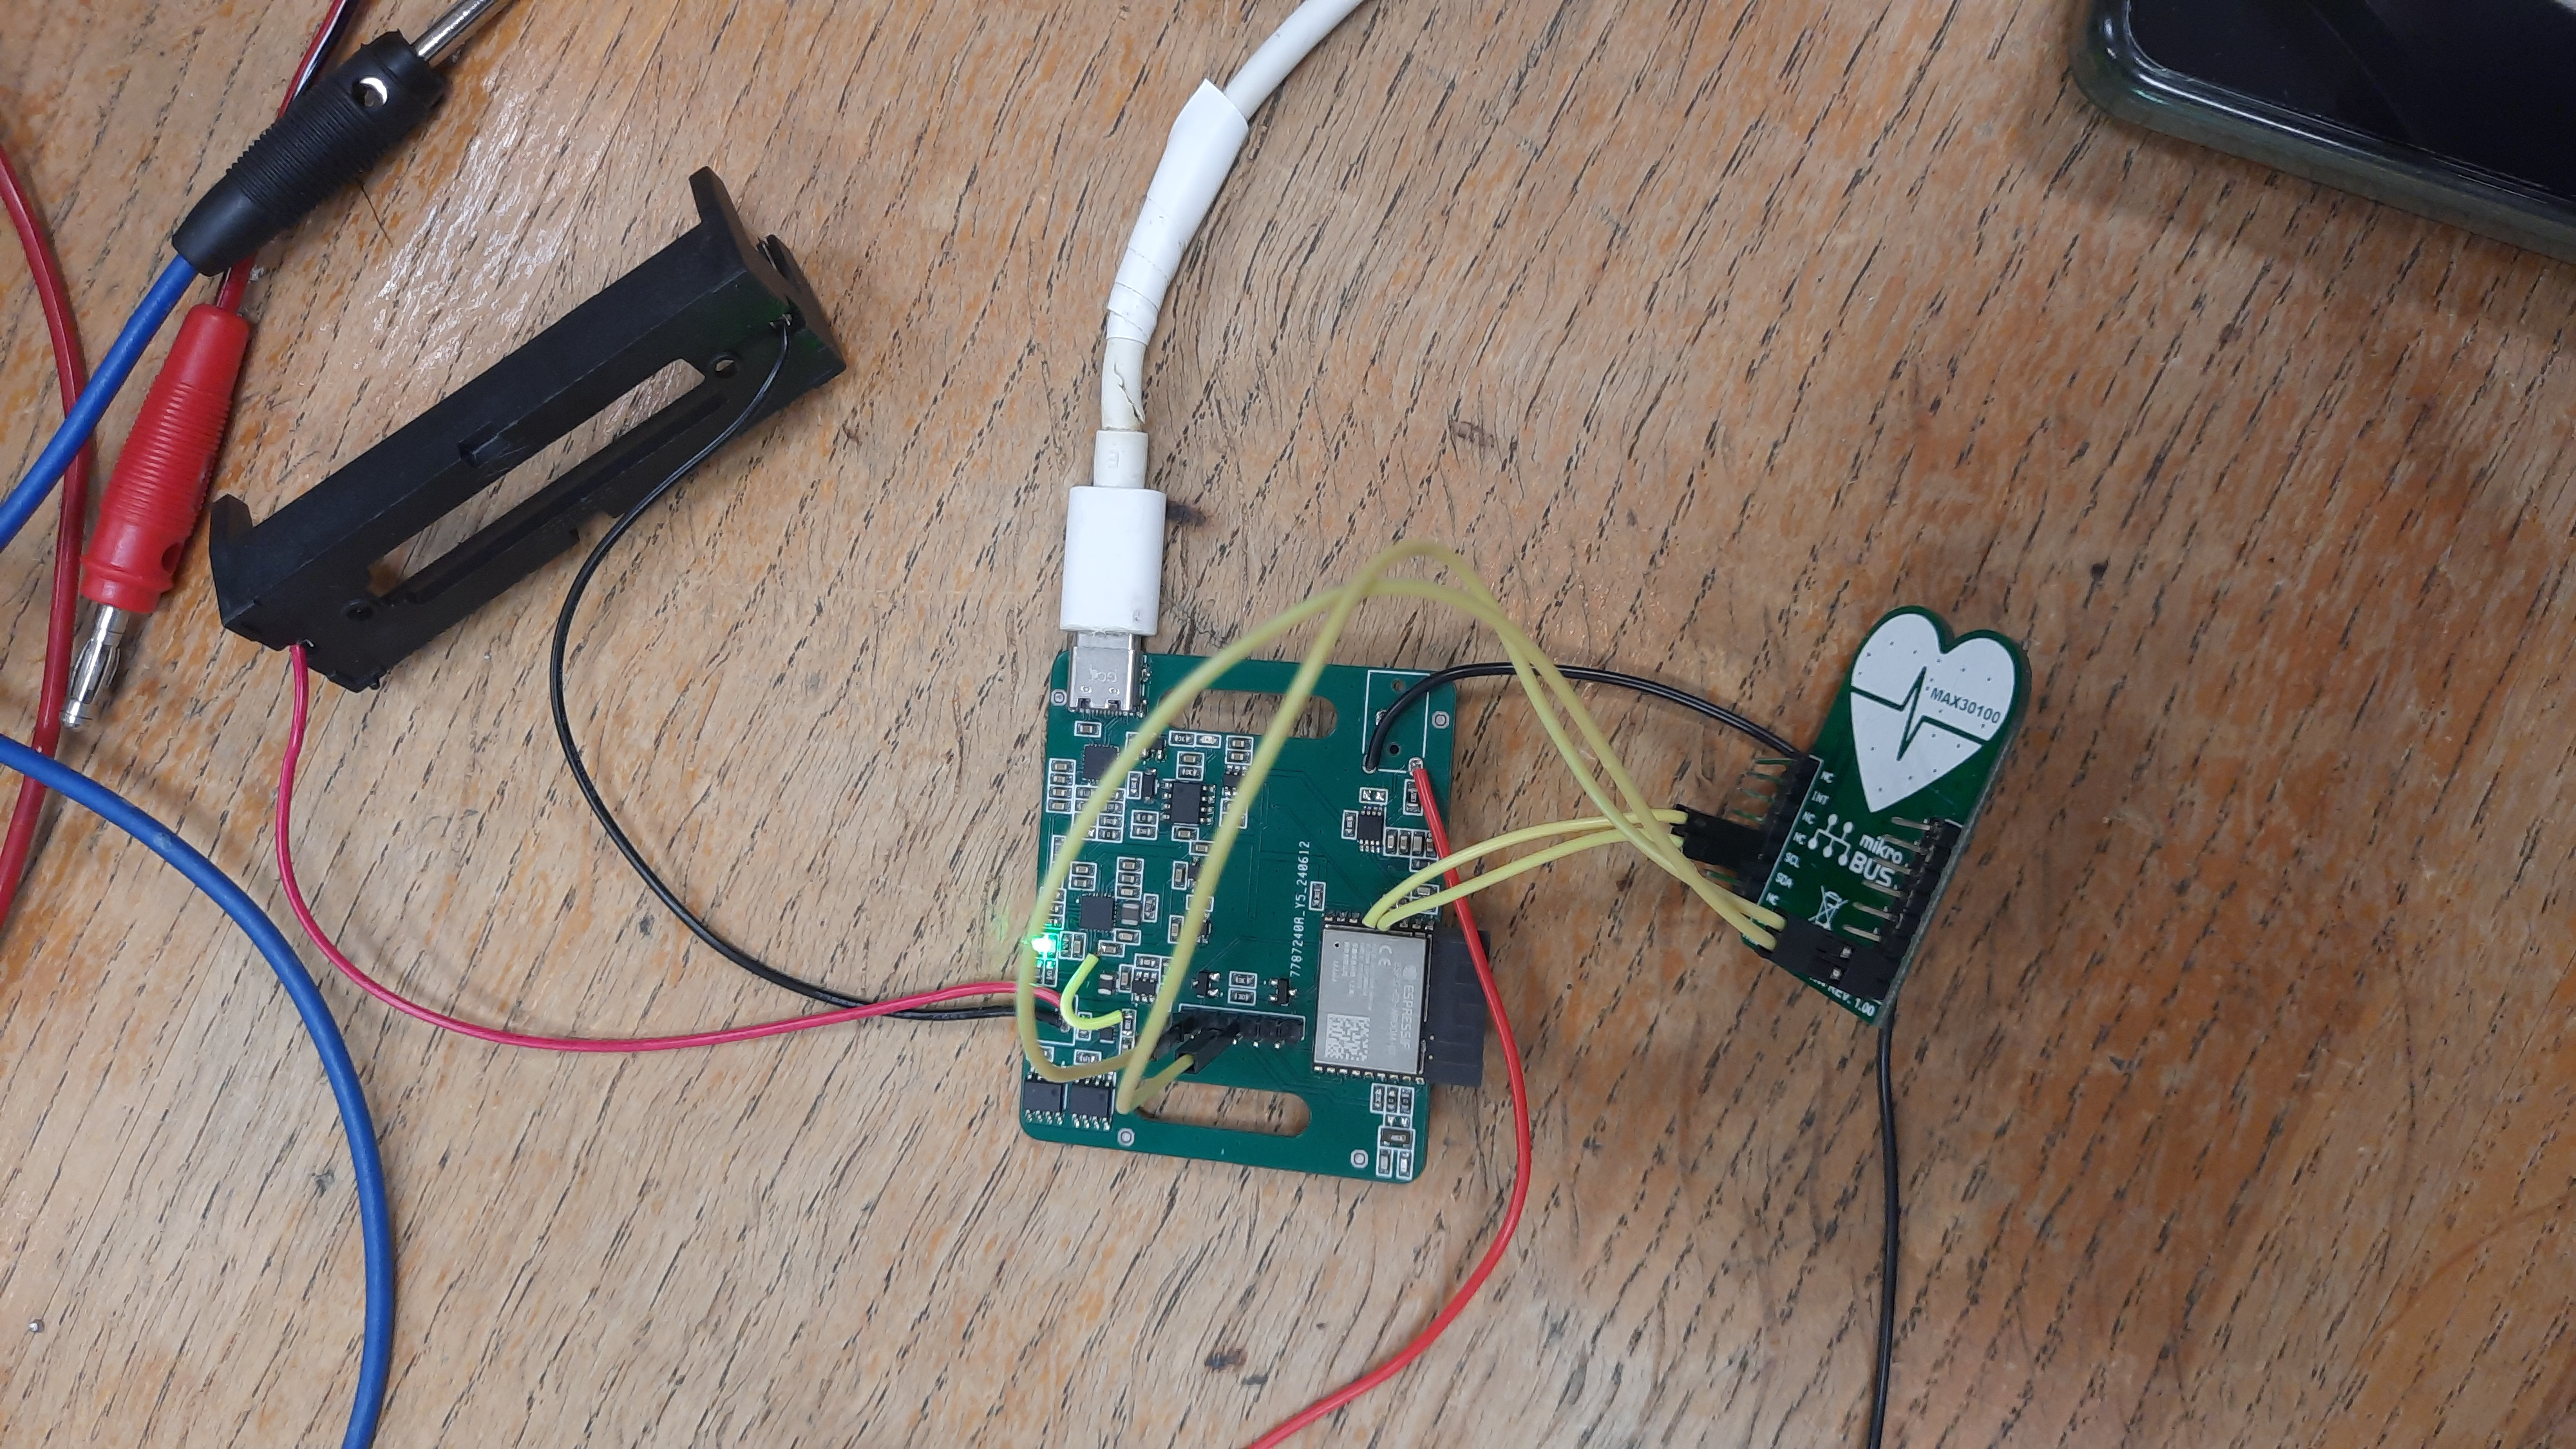
\includegraphics[width=10 cm]{Figures/BR_TEST_05.jpg}
    \caption{Spoj modula sa MAX30100 na pločicu}
    \label{slk:BR_TEST_05}
\end{figure}

ESP modul koji se nalazi na pločici programiran je putem USB sučelja.